%---------- Segundo Capítulo: Fundamentação --------------

\chapter{Fundamentação Teórica}
%10 --- 15 pags

%teorico - cientifico (mtas referencias aqui)

%introducao --- desenvolvimento --- considerações
%\section{Sistema Visual Humano}

\section{Vídeo Digital}
Imagem é um registro aproximado de um instante de tempo do mundo real, pois representa uma quantidade de informação limitada suficiente para que qualquer pessoa possa, posteriormente, reconhecer aquela representação assimilando-a à uma realidade. Primeiramente, imagens são registros porque contém em si a captura de cores num instante de tempo, que nada mais são que intensidades luminosas (ondas eletromagnéticas que o olho humano é capaz de perceber).

Imagens são registros aproximados, ou limitados, pois dependem da tecnologia que as obtém e manipulam: as cores nem sempre são fiéis, a iluminação pode acabar atrapalhando a nitidez e a saturação, etc. Por fim, imagens usualmente são registros suficientes porque costumam permitir sua associação a situações e formas reais por qualquer pessoa apesar de suas limitações.

A tecnologia na obtenção de imagens se expande a cada dia, seja aprimorando as técnicas já utilizadas, seja criando novas técnicas. Até algumas décadas atrás, a única forma de obtenção era a analógica: através de filmes sensíveis a luz que a ela deveriam ser expostos por um infinitésimo de segundo através de um obturador; fitas magnéticas, etc.

Para a obtenção de sinais digitais, o sinal analógico (uma imagem é um sinal analógico) deve ser submetido às fases de amostragem e quantização, em que uma amostra é gerada em um instante de tempo \cite{rehme}.

Atualmente a forma digital de captura de imagens e vídeos, criada no fim da década de 1960, está bastante difundida por causa das vantagens que oferece, entre elas:

\begin{itemize}
	\item editar, adicionar efeitos, corrigir imperfeições, enfim, a manipulação é mais fácil e algumas operações só podem ser realizadas neste formato;
	\item o arquivo não perde a qualidade ao longo do tempo, como acontece com fitas magnéticas e filmes, onde o meio de armazenamento afeta diretamente a qualidade do conteúdo;
	\item a cópia é fiel, não causando modificação no conteúdo;
	\item o custo de armazenamento tem se tornado cada vez mais baixo;
	\item a integração com outras tecnologias e equipamentos é mais simples;
	\item possibilidade de correção de erros a partir de checksums e redundância;
	\item possibilidade de compressão com ou sem perdas;
	\item a repetibilidade da informação, em qualquer momento.
\end{itemize}

Vídeos digitais nada mais são que sequência de imagens digitais, e todos os conceitos do segundo valem para o primeiro. O contrário pode não ser verdadeiro, uma vez que num vídeo a presença da variável tempo permite-lhe operações exclusivas, como por exemplo a compressão temporal ou codificação inter-frame, detalhada mais adiante.

A gama de aplicações de vídeos digitais é ampla. Alguns exemplos são: transmissão de TV, streaming via internet, exames médicos, uso pessoal, web cams, câmeras em celulares e smartphones, câmeras de segurança, cinema, imagens via satélite, entre outros.

As limitações da tecnologia digital residem na capacidade de armazenamento de dados digitais, velocidade de armazenamento, dispositivos de captura e até mesmo na capacidade humana (por exemplo, de diferenciar cores, tonalidades, etc). Essas limitações moldam a representação digital de imagens, que são formadas por pixels (menor estrutura representativa de cor). Desta forma, a informação que se pode agregar a cada pixel é limitada e, consequentemente, afeta diretamente a quantidade de cores que cada pixel pode assumir.

Antes de explicar sobre o processo de quantização que determinará o conteúdo de cada pixel e seu formato, é importante que o conceito de modelo de cores seja introduzido.

Um modelo de cores é um modelo matemático que associa números a cores, ou seja, é uma função matemática de tuplas, de normalmente três ou quatro variáveis, que representam cores no espaço correspondente.

Várias são as formas de construir um modelo de cores e dentre alguns deles estão: RGB (componentes red-green-blue) figura \ref{fig:rgbspace}, YUV (componentes luminância-crominância-crominância) figura \ref{fig:yuvspace}e CMYK (componentes cyan-magenta-yellow-black) figura \ref{fig:cmykspace}.

\begin{figure}[ht]
    \begin{minipage}[b]{0.3\linewidth}
        \centering
        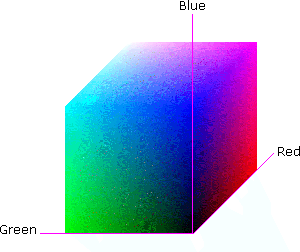
\includegraphics[width=\textwidth]{./imgs/rgbspace.png}
        \caption{RGB}
        \label{fig:rgbspace}
        \fonte{\cite{acasystems}}
    \end{minipage}
    \hspace{0.5cm}
    \begin{minipage}[b]{0.3\linewidth}
        \centering
        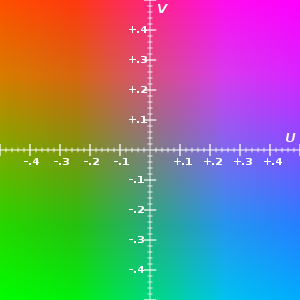
\includegraphics[width=\textwidth]{./imgs/yuvspace.png}
        \caption{YUV, para Y = 0.5}
        \label{fig:yuvspace}
        \fonte{\cite{wikiyuvspace}}
    \end{minipage}
    \hspace{0.5cm}
    \begin{minipage}[b]{0.3\linewidth}
        \centering
        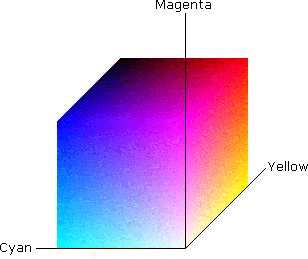
\includegraphics[width=\textwidth]{./imgs/cmykspace.png}
        \caption{CMYK}
        \label{fig:cmykspace}
        \fonte{\cite{acasystems}}
    \end{minipage}
\end{figure}

O modelo de cores RGB possui três componentes e a partir da combinação delas é possível criar uma infinidade de cores. Da mesma forma, o modelo de cores CMYK combina as componentes ciano, magenta, amarelo e preto para formar cores. Já no modelo YUV existe uma componente de luminância, ou brilho, e duas componentes de cor efetivamente (na realidade, essas componentes são respectivamente a diferença entre valores padrões de azul e vermelho e a luminância).

De posse destes conceitos iniciais, o significado de quantização torna-se mais simples. Numa imagem analógica, cada partícula da imagem pode assumir infinitos valores pois a intensidade luminosa registrada, por exemplo num filme, é uma grandeza física com domínio real. Já numa imagem digital, cada pixel deve ter uma quantidade finita de informação para que possa ser armazenado. Desta necessidade de se limitar o tamanho da informação surge o conceito de quantização: um espaço de cores é dividido em subespaços em que apenas uma cor o representa. Este processo pode ser visto como uma compressão com perdas, pois várias cores são perdidas.

Partindo-se da quantização, é necessário determinar a quantidade de bits por pixel (bpp ou profundidade de cor) que é equivalente ao número de níveis de intensidade de cada componente de cor do espaço de cores desejado. Por exemplo, utilizando-se 8 bits para cada componente do modelo RGB, o espaço de cores fica limitado a 256 valores para cada componente que, combinados, geram mais de 16 milhões de cores.

No espaço de cores RGB mostrado na figura \ref{fig:rgbdiscrete}, é possível observar o efeito da quantização. Os eixos, que a princípio tinham como domínio os reais, foram discretizados para assumir apenas valores inteiros não-negativos. Cada componente pode assumir seis valores e a combinação delas gera um total de 6\textsuperscript{3} = 216 cores. Desta forma, pode-se perceber que cada subespaço assumiu um único valor para representá-lo, ignorando as tonalidades de transição entre cada ponto do espaço.

\begin{figure}[!htb]
	\centering
	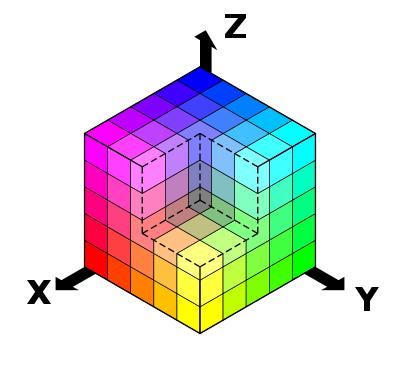
\includegraphics[width=0.5\textwidth]{./imgs/rgbdiscrete.png}
	\caption{Espaço RGB discretizado.}
	\label{fig:rgbdiscrete}
	\fonte{\cite{wikicolormodel}}
\end{figure}

A quantização e a quantidade de bits por pixel representam uma das vantagens da utilização de formatos digitais pois muita informação redundante aos olhos humanos (tons de cores muito próximos, por exemplo) pode ser removida. Neste aspecto, um ponto chave da fisiologia humana que favorece a compressão de imagens é o fato de a acuidade visual ser maior em relação à luminância do que à crominância \cite{vandenbranden}.

Um conceito importante que aproveita esta característica da visão humana é a subamostragem. Este conceito define que a resolução da camada de crominância pode ser menor que a resolução da camada de luminância, ou seja, para um conjunto de pixels, cada um possuirá seu valor de luminância, porém o de crominância poderá ser repetido, desta forma economizando recursos \cite{brice}. A figura \ref{fig:subsampling} apresenta, em colunas, alguns esquemas de subamostragem:

\begin{figure}[!htb]
	\centering
	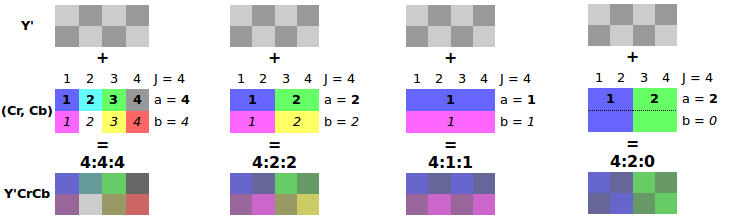
\includegraphics[width=0.9\textwidth]{./imgs/subsamplingschemes.png}
	\caption{Esquemas de subamostragem.}
	\label{fig:subsampling}
	\fonte{\cite{wikisubsampling}}
\end{figure}

Onde:
\begin{itemize}
	\item J - largura da amostra de referência, normalmente igual a 4;
	\item a - número de amostras de crominância (Cb, Cr) na primeira linha;
	\item b - número de amostras de crominância (Cb, Cr) na segunda linha.
\end{itemize}

O fator \emph{alpha} (coeficiente de opacidade) pode ser considerado na notação, mas normalmente é omitido por ter valor igual a J. A notação dos esquemas é obtida considerando-se J:a:b. Desta forma, no esquema 4:1:1 é obtida uma amostra de crominância para cada linha; no esquema 4:2:0 são obtidas duas amostras na primeira linha que serão repetidas na segunda; no esquema 4:2:2 uma amostra de crominância é feita para cada conjunto de dois pixels (na horizontal) e, por fim, no esquema 4:4:4 não há subamostragem, uma vez que a crominância é amostrada para cada pixel, não ocorrendo compressão por não haver possibilidade de repetição.

Em valores reais, considerando-se 24 bpp (8 para cada componente de crominância e 8 para a componente de luminância), uma imagem sem subamostragem (esquema 4:4:4) de dimensões 4x2, como a da figura, equivaleria à 24x4x2 = 192 bits. A tabela \ref{tab:subsampling}  sintetiza o valor em bits desta mesma imagem para cada esquema de subamostragem:

\begin{table}[!h]
	\centering
	\caption[Tamanho em bits para cada subamostragem]{Tamanho em bits da mesma imagem (4x2) para cada esquema de subamostragem.}
	\label{tab:subsampling}
	\begin{tabular}{|c|c|c|c|}
		\hline
		Esquema & Total de bits de luminância & Total de bits de Crominância & Total de bits \\
	    \hline
		4:4:4 & 8x4x2 = 64 & (8+8)x4x2 = 128 & 192 \\
	    \hline
		4:1:1 & 8x4x2 = 64 & (8+8)x2 = 32 & 96 \\
	    \hline
		4:2:0 & 8x4x2 = 64 & (8+8)x2 = 32 & 96 \\
	    \hline
		4:2:2 & 8x4x2 = 64 & (8+8)x2x2 = 64 & 128 \\
		\hline
	\end{tabular}
\end{table}

O vídeo digital com qualidade \emph{standard} (\sigla{SDTV}{Standard Definition Television}) é definido pela norma \sigla{SMPTE}{Society of Motion Picture and Television Engineers} 259M (Society of Motion Picture and Television Engineers). Possui dimensões de 720x480 pixels com esquema de subamostragem 4:2:2. O padrão de \sigla{DVD}{Digital Video Disk} (Digital Video Disk) utiliza o esquema 4:2:0 de subamostragem.

\subsection{Arquivo em formato bruto}

É possível armazenar diretamente os valores das amostras num arquivo. Este tipo de arquivo, conhecido como arquivo raw, ou bruto, não passa por qualquer processamento, codificação ou encapsulamento. Existe uma infinidade de formatos de arquivo de vídeo bruto, cada um com uma organização particular que ordena os valores das componentes de cada pixel, entre eles os formatos: AYUV, UYVY, CYUV, YUY2, Y41P, Y411, YUVP, Y211, YV16, YV9, Y800 \cite{fourccyuv}. %TODO precisa dessa jeba enorme de siglas?

A figura \ref{fig:yuvorganization} mostra a organização de um arquivo no formato IYUV (ou I420) de subamostragem 4:2:0 e o respectivo fluxo de bytes em memória. Primeiramente são armazenados os valores de luminância de cada pixel, os valores de crominância U (Cb) para cada conjunto de 4 pixels e os de crominância V (Cr) para o mesmo conjunto.

\begin{figure}[!htb]
	\centering
	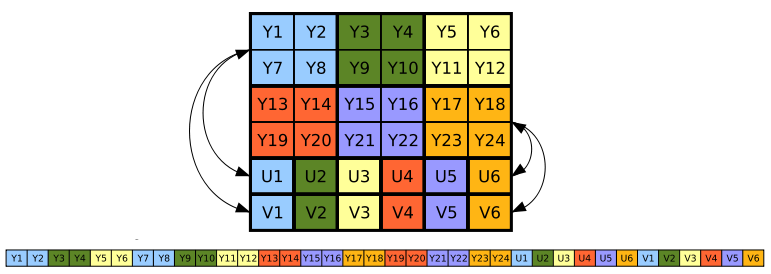
\includegraphics[width=0.9\textwidth]{./imgs/yuvorganization.png}
	\caption{Organização de um arquivo no formato YUV.}
	\label{fig:yuvorganization}
	\fonte{\cite{wikiyuvspace}}
\end{figure}

\section{Codificação}

O objetivo principal da codificação de vídeos é a compressão de dados que torna viável seu armazenamento e transmissão \cite{daronco}.

A codificação ou compressão é o processo que reduz o número de bits de dados digitais a fim de se diminuir a necessidade por recursos, tais como espaço de armazenamento e banda de transmissão. A compressão possui duas categorias básicas: pode ser sem perdas, isto é, apenas informações estatisticamente redundantes são removidas conservando a informação original; e pode ser com perdas, em que informações menos relevantes são descartadas pela necessidade imposta.

Um exemplo de como a compressão é importante atualmente pode ser verificado na transmissão de vídeos por streaming. Considerando-se apenas os valores de luminância (escala de cinza) de um vídeo com definição standard (SD - Standard Definition) de 640x480 pixels com 8 BPP, tem-se que cada quadro de imagem ocupa 8x640x480 = 2.45 Mbits de memória. Se o vídeo deve ser apresentado a uma taxa de 30 FPS (frames per second - quadros por segundo), a banda necessária para transmitir o vídeo deve ser de 30x2.45 Mbits/s = 73.50 Mbps. Adicionando-se informações de cor e de áudio, esta taxa chega facilmente aos 270 Mbps numa qualidade SD, e ultrapassa 1.4 Gbps numa qualidade HD (High Definition - alta definição), valores que teriam um custo impraticável para usuários domésticos e até mesmo para empresas \cite{ciscoieee}. A codificação permite que até 98\% do sinal digital original seja removido sem que haja uma degradação inaceitável na qualidade da imagem \cite{mpeg2ref}.

A Figura \ref{fig:codingprocess} apresenta o processo de obtenção, codificação (etapa A), transmissão, recepção e decodificação (etapa B) de um sinal de áudio e/ou vídeo sendo, por fim, apresentado. As etapas de conversão A/D (analógico-digital) e conversão D/A (digital-analógico) podem ser suprimidas caso a conversão A/D já seja realizada nos equipamentos de obtenção de dados e caso os monitores e dispositivos de armazenamento sejam digitais \cite{rehme}.

\begin{figure}[!htb]
	\centering
	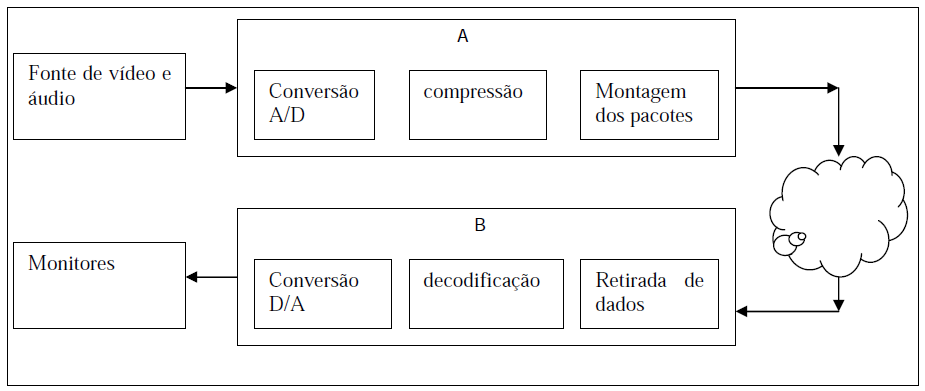
\includegraphics[width=0.9\textwidth]{./imgs/codingprocess.png}
	\caption{Etapas de codificação e decodificação.}
	\label{fig:codingprocess}
	\fonte{\cite{rehme}}
\end{figure}

As etapas gerais da compressão são:

\begin{itemize}
	\item obter as diferenças entre quadros;
	\item estimar movimento;
	\item realizar transformações nos domínios espacial e de frequência.
\end{itemize}

A compressão espacial opera num mesmo \emph{frame} e tem por objetivo remover possíveis redundâncias para diminuir a quantidade de dados que o representam. Já a compressão temporal opera numa sequência de \emph{frames}, buscando encontrar semelhanças entre eles, uma vez que em \emph{frames} sucessivos ocorrem poucas modificações, na maior parte do tempo. Desta forma, a parte do \emph{frame} que não sofreu alterações é repetida do anterior e apenas a parte modificada é efetivamente utilizada para descrever o \emph{frame} a ser apresentado.

De acordo com \cite{rehme}: “Para a compressão temporal, precisa-se de um ponto de partida ou quadro-chave. Depois dele, apenas as diferenças são descritas”.

Em relação aos mecanismos de codificação de fonte, \cite{rehme} afirma que “quanto mais sofisticados forem, normalmente melhor é a relação qualidade versus taxa de bits, porém apresentam maior custo em termos de capacidade de processamento e maior tempo requerido para executar a compressão. Para várias situações, o aumento do atraso entre a captura da imagem e sua apresentação não é tolerável”.

Percebe-se desta forma que existe um equilíbrio entre método e taxa de compressão, degradação da qualidade aceitável e recursos disponíveis, ambos dependentes da aplicação.

Em 1987, a International Electrotechnical Commission (IEC - Comissão Eletrotécnica Internacional) juntamente com a International Organization for Standardization (ISO - Organização Internacional para Padronização) organizou um grupo de especialistas com o objetivo de padronizar a compressão de áudio e vídeo digitais, mais conhecido como Moving Picture Experts Group, ou MPEG. Em seu primeiro encontro, realizado em 1988, após o sucesso da digitalização do sinal de áudio (de natureza analógica) e posterior compressão para o desenvolvimento do popular CD (com áudio de alta qualidade), percebeu-se que aplicar a ideia na transmissão de TV diminuiria a largura de banda necessária, possibilitando a emissão de programas interativos, serviços de internet e ainda mais programas \cite{mpeg2ref}.

O MPEG desenvolveu uma série de protocolos para as questões que surgiram ao longo do desenvolvimento de novas tecnologias, novos equipamentos e novos padrões internacionais, a fim de padronizar emissões digitais. Os padrões desenvolvidos incluem MPEG-1, MPEG-2, MPEG-4 e, mais recentemente, MPEG-7.

Atualmente, a indústria de transmissão de TV se baseia principalmente no padrão MPEG-2 para transmitir sinal de vídeo digital, áudio e dados pela rede. Este é o padrão para transmissão digital, pois é o único que prevê suporte a transmissão de dados via rede \cite{mpeg2ref}.

Os dois principais tipos de compressão do MPEG são as codificações espacial e temporal. O primeiro tipo elimina redundâncias entre pixels adjacentes num mesmo \emph{frame}, aproveitando-se, também, da inabilidade do olho detectar certas degradações. O segundo tipo minimiza redundâncias entre \emph{frames} \cite{mpeg2ref}.

O processo de codificação espacial envolve as seguintes etapas, segundo \cite{mpeg2ref}:
\begin{itemize}
    \item Transformada Discreta de Cossenos - \sigla{DCT}{Discrete Cosine Transform}: cada \emph{frame} é dividido em matrizes de dimensões 8x8 \emph{pixels} em que as intensidades luminosas serão transformadas em valores baseados em frequência, chamados coeficientes. Por causa da redundância espacial, muitos coeficientes resultam no valor zero, que podem ser eliminados da série de coeficientes. O resultado é uma compressão com perdas imperceptíveis ao olho humano, em que o mesmo \emph{frame} é representado por menos \emph{bits}.
    \item Quantização (\emph{Quantization}): os coeficientes da DCT são reorganizados em ordem de importância visual.
    \item Ponderação (\emph{Weighting}): degradação, ou ruído, são estrategicamente adicionados em regiões mais detalhadas ou complexas, onde é pouco provável que o observador note. 
    \item Varredura (\emph{Scanning}): nesta etapa os coeficientes mais significantes são enviados primeiro, seguidos dos menos importantes e, por fim, uma indicação de que os restantes são iguais a zero.
    \item Codificação de Entropia (\emph{Entropy Conding}): os coeficientes são reajustados de acordo com sua frequência de ocorrência. Os que mais se repetem são expressos com menor número de \emph{bits}, o que diminui consideravelmente a banda necessária para transmití-los.
\end{itemize}

Já a codificação temporal aproveita-se da similaridade entre \emph{frames} sequenciais, codificando apenas a diferença entre eles. Isso é possível devido a dois tipos de codificação temporal: previsão entre \emph{frames} e previsão de movimento (\emph{inter-frame prediction} e \emph{motion prediction}).

A previsão entre \emph{frames} codifica um \emph{frame} completo apenas periodicamente. O resultado, chamado de \emph{intra-coded frame} ou I-\emph{frame}, é utilizado como referência para \emph{frames} anteriores e posteriores.

\emph{Predicted Frames}, ou P-\emph{frames}, têm por referência um I-\emph{frame} ou um P-\emph{frame} anterior, ou seja, ao invés de transmitir todos os coeficientes DCT, o codificador transmite apenas aqueles coeficientes que sejam diferentes do I-\emph{frame} ou um P-\emph{frame} anterior. No outro lado, o decodificador reconstrói um P-\emph{frame} apenas aplicando as diferenças sobre o I-\emph{frame} ou P-\emph{frame} de referência \cite{mpeg2ref}.

\emph{Bidirectionally Predicted Frames}, ou B-\emph{frames}, podem utilizar tanto I-\emph{frames} ou P-\emph{frames} precedentes quanto subsequentes, como pode ser observado na Figura \ref{fig:ipbframes}. O I-\emph{frame} inicial é completamente codificado, já o P-\emph{frame} subsequente possui apenas a parte que sofreu modificação em relação ao I-\emph{frame} anterior. O B-\emph{frame} presente na figura, armazena as diferenças em relação ao P-\emph{frame} anterior e ao I-\emph{frame} seguinte.

\begin{figure}[!htb]
	\centering
	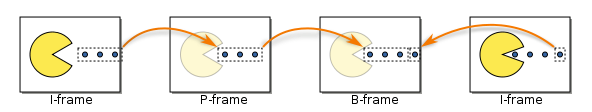
\includegraphics[width=0.9\textwidth]{./imgs/ipbframes.png}
	\caption{Estrutura de predição de \emph{frames} no MPEG.}
	\label{fig:ipbframes}
	\fonte{\cite{wikiipbframes}}
\end{figure}

P-\emph{frames} alcançam uma compressão maior que I-\emph{frames}, tipicamente de 20\% a 70\% do tamanho do respectivo I-\emph{frame} de referência. B-\emph{frames}, por sua vez, podem permitem uma compressão ainda maior, tipicamente de 5\% a 40\% do tamanho do respectivo I-\emph{frame} de referência \cite{ciscoieee}.

Apesar de reduzir a quantidade de informação a ser transmitida, quanto menos I-\emph{frames} são utilizados, maior é a vulnerabilidade da transmissão. Qualquer erro que ocorrer num I-\emph{frame} será propagado até que um novo seja enviado corretamente  cite{mpeg2ref}. Por este motivo o conceito de \sigla{GOP}{Group Of Pictures} (\emph{Group Of Pictures}) é utilizado \cite{mpeg2ref}. Cada conjunto é iniciado por um I-\emph{frame}, contendo também P-\emph{frames} e B-\emph{frames}.

O tamanho usual para um GOP é entre 12 e 15 \emph{frames} \cite{ciscoieee, mpeg2ref}. Um exemplo de GOP pode ser observado na Figura \ref{fig:gop}.

\begin{figure}[!htb]
	\centering
	
\includegraphics[width=0.9\textwidth]{./imgs/gop.png}
	\caption{Estrutura de um GOP.}
	\label{fig:gop}
	\fonte{\cite{ciscoieee}}
\end{figure}

A previsão de movimento, por sua vez, envia um vetor de movimento (\emph{motion vector}) para o decodificador. Este vetor resulta da identificação de movimento de objetos que se repetem, desta forma, o decodificador apenas move o objeto para a nova posição.

Para que seja possível transportar vídeos codificados com MPEG por uma rede \sigla{IP}{Internet Protocol}, a informação dos \emph{frames} deve ser encapsulada em pacotes MPEG-\sigla{TS}{Transport Stream}, que serão transportados por pacotes IP posteriormente \cite{ciscoieee}. Pacotes IP contém sete pacotes MPEG-TS de 188 \emph{bytes}. 

A Figura \ref{fig:ts} apresenta o encapsulamento típico de um pacote IP. Cada pacote pode conter informação de dois \emph{frames} consecutivos, ou seja, a perda de um pacote pode trazer a perda de informação referente aos dois \emph{frames}. Vale observar que além de informações de imagem, os pacotes IP também transportam informações de áudio codificado em MPEG e informações de serviço \cite{ciscoieee}.

\begin{figure}[!htb]
	\centering
	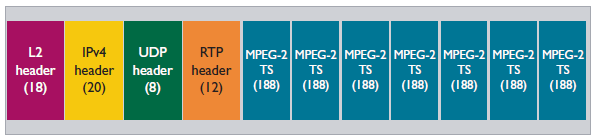
\includegraphics[width=0.9\textwidth]{./imgs/ts.png}
	\caption{Estrutura de pacote IP.}
	\label{fig:ts}
	\fonte{\cite{ciscoieee}}
\end{figure}

\section{Artefatos}

Imagens digitais são alvo de uma grande variedade de distorções durante sua aquisição, processamento, compressão, armazenamento, transmissão e reprodução \cite{wangbovik2004}. As características peculiares que são observadas nas imagens são chamadas de artefatos \cite{albini} e podem ser observadas tanto em transmissões digitais quanto em transmissões analógicas.

As imagens digitalmente transmitidas, embora suscetíveis à um grande número de distorções, não sofrem as mesmas distorções que as convencionais, de transmissão analógica (salvo no caso de um sinal analógico ser convertido para ser transmitido em meio digital). O ruído branco gaussiano é um exemplo de distorção que ocorre em meio analógico e podm ser observado na Figura~\ref{fig:artefatosanalogicos} a seguir:

\begin{figure}[!htb]
	\centering
	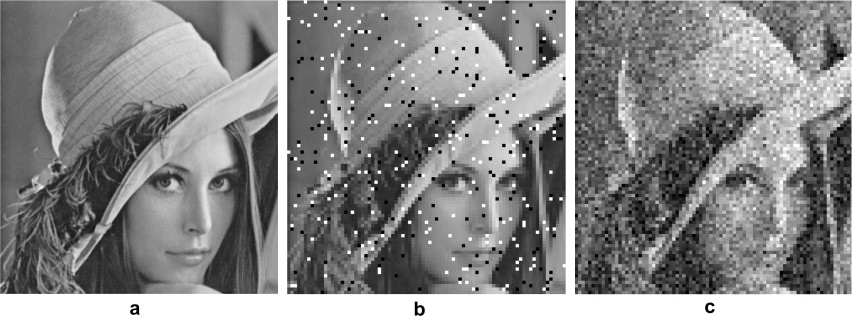
\includegraphics[width=0.9\textwidth]{./imgs/artefatosanalogicos.png}
	\caption{Ruído branco gaussiano.}
	\label{fig:artefatosanalogicos}
	\fonte{\cite{panagiotopoulou}}
\end{figure}

Em se tratando de vídeos digitais, os artefatos de maior notoriedade são: \emph{blockiness}, \emph{blurriness}, \emph{ringing}, e \emph{noisiness} \cite{farias2007} e podem ser observados na Figura~\ref{fig:artefatosdigitais}, a seguir:

\begin{figure}[!htb]
	\centering
	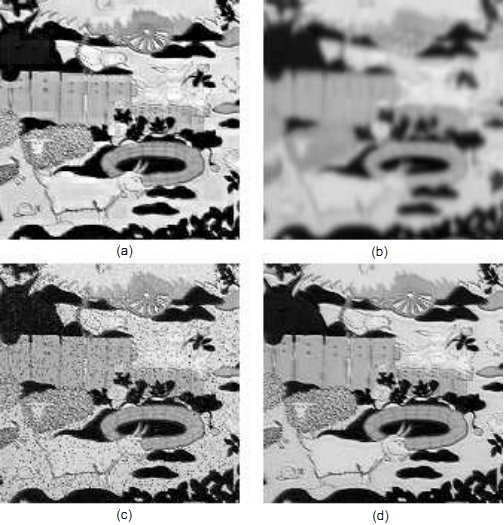
\includegraphics[width=0.9\textwidth]{./imgs/artefatosdigitais.png}
	\caption[Artefatos digitais]{Artefatos digitais (a) blocagem; (b) borramento; (c) \emph{noiseness} e (d) \emph{ringing}.}
	\label{fig:artefatosdigitais}
	\fonte{\cite{farias2007}}
\end{figure}

Poder adicionar artefatos de forma artificial e controlada à vídeos digitais é de grande importância no campo de avaliação de vídeos (tanto na avaliação objetiva quanto na avaliação subjetiva) uma vez que, a partir de algoritmos, é possível simular distorções reais. Estes algoritmos não são padronizados, mas existem algumas recomendações internacionais, como por exemplo a recomendação P.930 da ITU \cite{itup930} que descreve os princípios para reproduzir as distorções relativas à compressão de vídeo sem efetivamente precisar comprimí-lo.

Nas seções que seguem, alguns dos artefatos mais comuns serão detalhados juntamente com as recomendações para a respectiva simulação.

\subsection{Efeito de Blocagem - \emph{Blocking effect}}

Este artefato é o mais estudado pela literatura \cite{emmersonsilva}. Ocorre em função de uma quantização grosseira no processo de compressão, em que resulta numa distorção ou perda de componentes de alta frequência \cite{itup930}. Normalmente ocorre em superfícies lisas em movimento \cite{itup930} \cite{farias2007}.

A recomendação P.930 indica que a simulação deste artefato deve, primeiramente, localizar regiões de movimento em uma imagem para posteriormente selecionar em quais possíveis janelas será aplicada uma média dos valores de luminância \cite{itup930}. Desta forma, o cálculo da DCT e todo o processo de compressão é evitado.

\subsection{Efeito de Borramento - \emph{Blurring effect}}

O artefato de borramento é, visualmente, a perda de nitidez das bordas e de detalhes espaciais em uma imagem, como em áreas com texturas ou ao redor das bordas de objeto de cena \cite{wurao2005}. É causado pelo algoritmo de compressão no momento em que escolhe codificar bits de resolução ou de movimento \cite{itup930}.

A recomendação P.930 fornece os filtros a serem utilizados para a simulação deste artefato.

\subsection{Efeito de Travamento - \emph{Jerkiness}}

Este artefato é facilmente percebido em sistemas com baixa taxa de bits para vídeo, como em sistemas de teleconferência \cite{itup930} em que a imagem parece congelar em determinados instantes. Isso se deve à repetição de \emph{frames} com o objetivo de reduzir a quantidade de informação a ser transmitida ou processada \cite{itup930}.

A recomendação P.930 fornece dois fatores para controlar as repetições numa simulação: o FRF (Frame Repetition Factor) e o EFR (Effective Frame Rate). Um FRF igual a 3 causa a repetição do terceiro \emph{frame} de uma sequência durante os próximos dois \emph{frames}. O EFR é calculado como 30/FRF, e para o exemplo dado tem valor de 10 FPS.

\section{Métricas de Avaliação}

A compressão tende a diminuir a fidelidade, ou seja, o problema da codificação é encontrar um equilíbrio entre o nível de compressão necessário para transmitir pelo canal e o nível de fidelidade que se deseja exibir para o espectador \cite{daronco}.

Apesar de a transmissão digital garantir que a interferência à ruídos seja mínima, a qualidade da imagem não depende somente de interferência, como foi visto. A compressão de vídeos é excelente na perspectiva do transmissor já que o custo do equipamento torna-se menor, porém na perspectiva do receptor/usuário a compressão pode comprometer muito a qualidade.

Neste contexto de tentar equilibrar qualidade e compressão, surge a necessidade de se criarem métodos capazes de avaliar a qualidade dos vídeos transmitidos tanto da parte dos emissores, para saber até que ponto a compressão não é percebida pelo usuário, ou pelo menos que ela não o incomode a ponto de deixar de assistir a transmissão; quanto da parte do usuário, que colabora para ter um serviço melhor.

Diversas metodologias definidas em normas internacionais foram criadas para avaliar a qualidade da informação multimídia (tanto áudio quanto vídeo), divididas em dois paradigmas: avaliação objetiva e avaliação subjetiva, descritas a seguir.

\subsection{Métricas Objetivas}

A avaliação objetiva tenta, através de algoritmos, fazer uma previsão aproximada da qualidade observada pelos observadores \cite{albini}. Os métodos mais simples e mais difundidos são definidos estatisticamente como o MSE (Mean Squared Error - Erro Médio Quadrático) e o PSNR (Peak Signal to Noise Ratio - Razão Sinal-Ruído de Pico) \cite{emmersonsilva} entre os dados originais e os dados recebidos (no caso de vídeos, o cálculo é aplicado pixel a pixel).

Outra métrica objetiva, o SSIM (Structural SIMilarity Index - Indice de Similaridade Estrutural), foi elaborado na tentativa de se aproximar a avaliação às percepções do SVH, pois leva em consideração a luminância, estrutura e o contraste (SILVA). Uma métrica derivada do SSIM é o MSSIM (Mean Structural SIMilarity Index - Indice de Similaridade Estrutural Média), sendo uma média dos valores SSIM calculados a partir do vídeo avaliado (WANG et al, 2004).

\subsubsection[MSE]{MSE - Mean Squared Error}

O MSE é a média das diferenças ao quadrado entre os valores de nivel de cinza dos pixels. Considerando que o nível de cinza de cada pixel é dado em função de sua posição de acordo com a equação a seguir:

Equação: G = f(t, x, y), onde:

\begin{itemize}
	\item G = nivel de cinza do pixel, dada sua posição;
	\item t = frame onde o pixel está localizado;
	\item x = posição relativa ao eixo vertical no frame;
	\item y = posição relativa ao eixo horizontal no frame.
\end{itemize}

o MSE pode ser calculado conforme a seguinte equação:

    Equação: \[MSE = \frac{1}{\left (T \cdot X \cdot Y \right )} \sum_{t}^{T} \sum_{x}^{X} \sum_{y}^{Y} \left ( P_{1} - P_{2} \right )^{2}\]

para vídeos com T \emph{frames} de tamanho X x Y \cite{winkler2005}.

    Conforme a medida obtida, a seguinte análise é feita: quanto menor o valor do MSE, mais próxima a imagem avaliada está da imagem original \cite{albini}. A imagem da função MSE é o conjunto dos reais, maiores ou iguais a zero, ou seja, um valor zero indica que as imagens são idênticas.

\subsubsection[PSNR]{PSNR - Peak Signal to Noise Ratio}
O PSNR é calculado com base num valor MSE e é dado em escala logarítmica. O PSNR mede a fidelidade entre imagens, ao contrário do MSE que mede diferenças entre imagens \cite{winkler2005}. Esta medida é encontrada conforme a equação a seguir:

Equação: \[PSNR_{dB} = 10 \cdot log_{10} \frac{{\left(2^{n} -1 \right )}^{2}}{MSE}\]

onde n é o número de bits que representa o nível de cinza de cada pixel.

A popularidade na utilização desta métrica se deve ao fato de que o cálculo pode ser realizado rapidamente, sendo bastante utilizado para comparar vídeos comprimidos e descomprimidos \cite{emmersonsilva, richardson2003}.

Dentre as limitações desta métrica, está a necessidade de sincronização entre as imagens original e degradada, baixa correlação com as métricas subjetivas definidas na norma ITU-R \cite{emmersonsilva, itubt500}.

Analisando os resultados, valores de PSNR altos indicam alta fidelidade entre as imagens comparadas, enquanto que valores baixos indicam baixa fidelidade.

\subsubsection[SSIM]{SSIM - Structural Similarity Index}

Esta métrica surgiu com o objetivo de melhor aproximar a avaliação objetiva à percepção humana, pois métricas como o MSE e o PSNR se mostraram ineficientes para tanto \cite{emmersonsilva}. Aplicado sobre valores de luminância, contraste e a estrutura para várias janelas de mesmas dimensões em uma imagem \cite{wangbovik2004}, tem como equação:

    Equação: \[SSIM(x, y) = \frac{(2\mu_{x}\mu_{y} + C_{1})(2\sigma_{xy} + C_{2})} {(\mu_{x}^{2} + \mu_{y}^{2}+C_{1})(\sigma_{x}^{2} + \sigma_{y}^{2}+C_{2})}\]

onde:
\begin{itemize}
	\item x e y são janelas sendo comparadas de dimensões NxN;
	\item \(\mu_{x}\) é a média de x;
    \item \(\mu_{y}\) é  a média de y;
    \item \(\sigma^{2}_{x}\) é a variância de x;
    \item \(\sigma^{2}_{y}\) é a variância de y;
    \item \(\sigma_{xy}\) é a covariância de x e y;
    \item C1 = \((k_{1}L)^{2}\), C2 = \((k_{2}L)^{2}\) são duas variáveis para estabilizar a divisão;
    \item L é a faixa dinâmica dos valores dos pixels (normalmente é \(2^{bits por pixel} - 1\));
    \item \(k_{1}\) = 0.01 e \(k_{2}\) = 0.03. Estes são valores são indicados pelos autores do método \cite{wangbovik2004} em decorrência de experimentos realizados.
\end{itemize}

\subsubsection[MSSIM]{MSSIM - Mean Structural Similarity Index}

Em termos práticos, normalmente é desejado encontrar-se uma medida de qualidade geral de toda a imagem \cite{wangbovik2004}. Por esta razão, a média dos índices SSIM é calculada:

Equação: \[MSSIM(X, Y) = \frac{1}{M} \sum_{i=1}^{M} SSIM(x_{j}, y_{j})\]

onde:
\begin{itemize}
	\item X e Y são as imagens de referência e distorcida, respectivamente;
	\item \(x_{j}\) e \(y_{j}\) são as janelas dentro das imagens;
	\item M é o número total de janelas na imagem.
\end{itemize}

\subsection{Métricas Subjetivas}

Por causa das limitações das métricas objetivas, muitos trabalhos foram realizados nos últimos anos para tentar desenvolver um teste objetivo mais sofisticado que se aproximasse dos resultados subjetivos \cite{watson1999, wangbovik2004}. Embora muitas métricas tenham sido propostas, nenhuma ofereceu um nível de qualidade em comparação aos testes subjetivos \cite{vqeg2003}.

A avaliação subjetiva depende de observadores humanos que atribuem notas a partir de suas opiniões sobre a qualidade. Posteriormente, uma análise estatística dos dados coletados é realizada, resultando em uma nota chamada MOS (Mean Opinion Score) \cite{itup930} \cite{albini}. Estes tipos de avaliação possuem algumas recomendações estabelecidas por órgãos internacionais com a finalidade de padronizar os procedimentos e ambientes de avaliação, alguns exemplos destas normas podem ser observados na Tabela \ref{tab:recomendacoes}:

\begin{table}
	\centering
	\caption{Recomendações da ITU}
	\label{tab:recomendacoes}
	\begin{tabular}{c|l}
		\hline
		\textbf{Nome da Norma} & Descrição \\
		\hline
		\textbf{ITU-R Rec. BT.500} & Metodologias para avaliação subjetiva da qualidade de vídeos \\
			& em televisores \\
		\textbf{ITU-T Rec. P.910} & Métodos para avaliação subjetiva de vídeos em aplicações \\
			& multimídia \\
		\textbf{ITU-T Rec. P.911} & Métodos para avaliação subjetiva de dados audiovisuais em \\
			& aplicações multimídia \\
		\textbf{ITU-T J.144} & Técnicas para avaliação objetiva de vídeo para televisão a cabo na \\
			& na presença de uma referência \\
		\textbf{ITU-R BS.1387} & Avaliação de sistema de áudio de alta qualidade. \\
		\hline
	\end{tabular}
	\fonte{\cite{daronco}}
\end{table}

As metodologias de avaliação seguem diretrizes que dizem respeito aos critérios para escolha das sequências de imagens, à seleção de observadores, a duração das sessões de avaliação, ao tempo de exposição de cada sequência e intervalos de troca, às condições ambiente, etc.

\subsubsection[Método DSIS]{Método DSIS - Double Stimulus Impairment Scale (Método EBU)}

Comumente usado para avaliação de novos sistemas ou dos prejuízos decorrentes de transmissão. Neste método, ao avaliador é apresentada uma imagem de referência e posteriormente a mesma imagem degradada. As sessões, que devem durar até 30 minutos, podem seguir duas variantes: na primeira, o conjunto referência/degradada é apresentado e ao final o avaliador deve dar uma nota. Na segunda variante, o avaliador é submetido duas vezes ao conjunto referência/degradada e somente ao final lhe é permitido dar a nota. Em ambas a apresentação dos conjuntos referência/degradada é aleatória.

A Figura \ref{fig:dsisvariantes} apresenta as fases de apresentação para cada variante. Em T1 e T3 o avaliador deve observar as imagens. O período T2 é de transição, deve ser apresentada uma tela cinza por 3 segundos. Por fim, o período T4 é o de avaliação, onde o avaliador efetivamente pode dar a nota. A Tabela \ref{tab:dsisfases} sintetiza as fases e os períodos recomendados.

\begin{figure}[!htb]
	\centering
	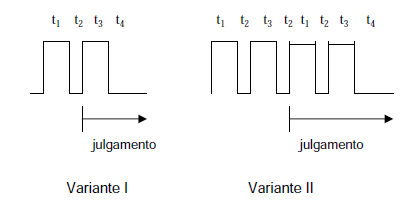
\includegraphics[width=0.9\textwidth]{./imgs/dsisvariantes.png}
	\caption{Variantes de aplicação da métrica DSIS.}
	\label{fig:dsisvariantes}
	\fonte{Adaptado de \cite{itubt500}}
\end{figure}

\begin{table}
	\centering
	\caption{Fases DSIS}
	\label{tab:dsisfases}
	\begin{tabular}{c|l}
		\hline
		\textbf{T1 = 10 s} & Imagem de referência \\
		\textbf{T2 = 3 s} & Cinza intermediário, nível de vídeo 200mV \\
		\textbf{T3 = 10 s} & Imagem degradada \\
		\textbf{T4 = 5-11 s} & Cinza intermediário \\
		\hline
	\end{tabular}
	\fonte{\cite{itubt500}}
\end{table}

A escala de avaliação a ser utilizada é dada conforme a Tabela \ref{tab:dsisescala}.

\begin{table}
	\centering
	\caption{Escala de avaliação DSIS}
	\label{tab:dsisescala}
	\begin{tabular}{c|l}
		\hline
		\textbf{5} & Imperceptível \\
		\textbf{4} & Perceptível, mas não irritante \\
		\textbf{3} & Pouco incômoda \\
		\textbf{2} & Irritante \\
		\textbf{1} & Bastante Irritante \\
		\hline
	\end{tabular}
	\fonte{\cite{itubt500}}
\end{table}

\subsubsection[Método DSCQS]{Método DSCQS - Double Stimiulus Continuous Quality Scale}

Este método também é aplicável para avaliar os efeitos dos meios de transmissão sobre a qualidade da imagem. Assim como no método DSIS, as imagens são apresentadas aos pares. Uma deve ser a imagem original e a outra deve ser a imagem processada pelo sistema em teste. A ordem de qual será apresentada por primeiro, bem como a ordem de apresentação de cada par, é aleatória. Outra diferença do método DSIS está na avaliação: o avaliador deve dar nota para ambas as imagens.

O número de repetições dos vídeos depende da duração da sequência de teste. Cenas mais estáticas devem durar de 3 a 4 segundos, podendo ser repetidas 5 vezes (as duas últimas são avaliadas), já cenas mais dinâmicas, que possuam artefatos variantes no tempo, devem durar 10 segundos e ser repetidas duas vezes (a segunda é avaliada).

As fases da apresentação DSCQS podem ser observadas na Figura \ref{fig:dscqsfases}. Elas são semelhantes as fases do método DSIS, a diferença está no momento em que a avaliação é permitida. 

\begin{figure}[!htb]
	\centering
	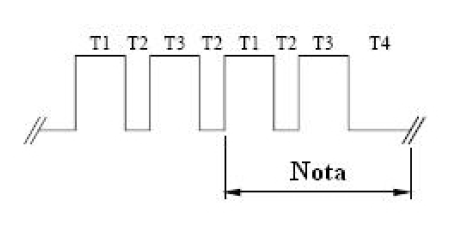
\includegraphics[width=0.9\textwidth]{./imgs/dscqsfases.png}
	\caption{Fases de apresentação do método DSCQS.}
	\label{fig:dscqsfases}
	\fonte{Adaptado de \cite{itubt500}}
\end{figure}

\begin{table}
	\centering
	\caption{Fases DSCQS}
	\label{tab:dsisfases}
	\begin{tabular}{c|l}
		\hline
		\textbf{T1 = 10 s} & Vídeo de teste A \\
		\textbf{T2 = 3 s} & Cinza intermediário, nível de vídeo 200mV \\
		\textbf{T3 = 10 s} & Vídeo de teste B \\
		\textbf{T4 = 5-11 s} & Cinza intermediário \\
		\hline
	\end{tabular}
	\fonte{\cite{itubt500}}
\end{table}

Para realizar a avaliação, o avaliador deve marcar as notas em uma escala contínua conforme a apresentada na Figura \ref{fig:dscqsescala}.

\begin{figure}[!htb]
	\centering
	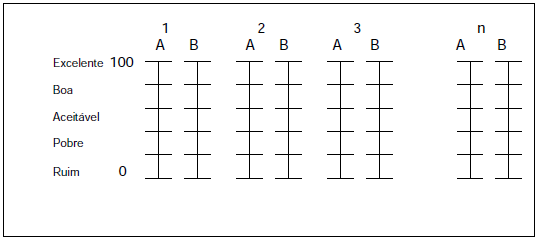
\includegraphics[width=0.9\textwidth]{./imgs/dscqsescala.png}
	\caption{Escala de avaliação da métrica DSCQS.}
	\label{fig:dscqsescala}
	\fonte{Adaptado de \cite{itubt500}}
\end{figure}

\subsubsection[Método SSCQE]{Método SSCQE - Single Stimulus Continuous Quality Evaluation}

Neste método, uma série de segmentos de programa são apresentados ao grupo de avaliadores com duração mínima de cinco minutos. Assim como no método DSCQS, a escala de avaliação é contínua. Os avaliadores modificam a nota conforme desejarem ao longo da apresentação das sequências. As notas, que são amostradas duas vezes por segundo, permitem o levantamento de histogramas \cite{rehme}.

Este método é mais adequado para avaliar a qualidade de vídeo em sequências longas e sem referência, o que é mais próximo da realidade.

\subsubsection[Método SDSCE]{Método SDSCE - Simultaneous Double Stimulus for Continuous Evaluation Method}

Para este método, as sequências de referência e de teste são apresentadas de forma simultânea. O avaliador deve julgar a fidelidade do vídeo em teste utilizando a escala contínua, assim como nos métodos DSCQS e SSCQE. A Figura \ref{fig:sdsce} demonstra como deve ser realizada a apresentação.

\begin{figure}[!htb]
	\centering
	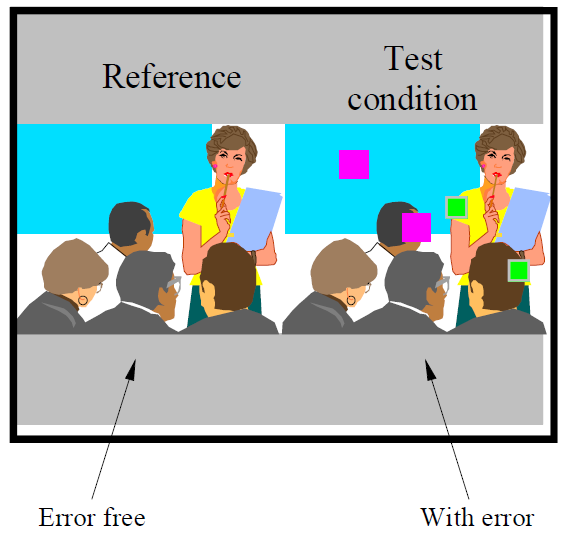
\includegraphics[width=0.9\textwidth]{./imgs/sdsce.png}
	\caption{Sessão de apresentação SDSCE.}
	\label{fig:sdsce}
	\fonte{\cite{itubt500}}
\end{figure}

As sequências podem ser apresentadas lado a lado no mesmo monitor ou em monitores diferentes, desde que tenham as mesmas especificações e características.

\section{Distribuições de Probabilidade}

Distribuição de probabilidade é um conceito fundamental em Estatística, utilizado em nível prático e teórico \cite{distteoria}.

As distribuições de probabilidade são funções matemáticas que mapeiam para todo valor dentro de um intervalo definido (discreto ou contínuo), valores de probabilidade de ocorrência, considerando uma variável aleatória que pode assumir qualquer valor deste intervalo\cite{distteoria}. Em outras palavras, é a função que descreve a probabilidade de uma variável aleatória assumir determinados valores \cite{wikidistribuicoes}.
 
Distribuições discretas são funções de probabilidade cuja variável pode assumir um número discreto de valores, não necessariamente finito. A definição matemática de uma função de probabilidade discreta, p(x), é uma função que satisfaz as seguintes propriedades:

\begin{itemize}
	\item A probabilidade de x assumir um valor específico é p(x);
	\item p(x) é não negativa para todo x real;
	\item a soma de p(x) para todos os valores possíveis de x é igual a 1.
\end{itemize}

Distribuições contínuas ou funções de probabilidade contínua são definidas para infinitos valores dentro de um intervalo. Por este fato, a probabilidade é medida para subintervalos, uma vez que a probabilidade de qualquer ponto é sempre zero\cite{distteoria}.

A definição matemática de uma função de probabilidade contínua, f(x), é uma função que satisfaz as seguintes propriedades:

\begin{itemize}
	\item a probabilidade de x estar entre dois pontos a e b é: \(p[a \leqslant x \leqslant b] = \int_{a}^{b}f(x)dx\);
	\item a probabilidade é sempre não-negativa para todo x real;
	\item a integral da função de probabilidade é: \(\int_{-\infty}^{\infty}f(x)dx = 1\)
\end{itemize}

Normalmente, distribuições de probabilidade são definidas por suas funções densidade de probabilidade, que associam a cada valor de x, sua probabilidade de ocorrência, de acordo com a equação a seguir: 

Equação: \(f(x) = Pr[X = x]\).

Particularmente para distribuições contínuas, a densidade de probabilidade é definida como a integral entre dois pontos, já que para qualquer ponto a probabilidade deve ser zero, como já descrito:

Equação: \(\int_{a}^{b}f(x)dx = Pr[a \leqslant X \leqslant b]\).

Algumas distribuições de probabilidade bastante conhecidas, como por exemplo a distribuição normal e a uniforme, são detalhadas a seguir.

\subsection{Distribuição Uniforme}

Distribuição uniforme contínua, ou distribuição retangular, é aquela em que todos os intervalos de mesmo tamanho tem a mesma probabilidade de ocorrer \cite{wikidistuniform1}. Mais precisamente, a probabilidade de se gerar qualquer ponto em um intervalo contindo no espaço amostral é proporcional ao tamanho do intervalo \cite{wikidistuniform2}. Em uma distribuição uniforme discreta, para todos os elementos possíveis a probabilidade é a mesma.

A equação da função densidade de probabilidade contínua dada a seguir, é exemplificada na Figura \ref{fig:uniformdist}.

Equação: \[\left\{\begin{matrix}
\frac{1}{(b-a)} & \mbox{para } a \leqslant x \leqslant b,\\ 
0 & \mbox{para } x < a \mbox{ ou } x > b
\end{matrix}\right.\]

\begin{figure}[!htb]
	\centering
	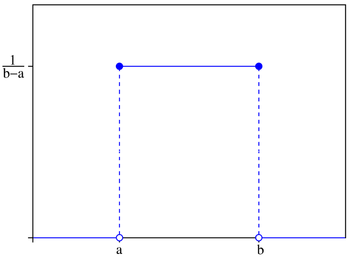
\includegraphics[width=0.9\textwidth]{./imgs/uniformdist.png}
	\caption{Função Densidade de Probabilidade de Distribuição Uniforme.}
	\label{fig:uniformdist}
	\fonte{\cite{wikidistuniform1}}
\end{figure}

Uma distribuição uniforme que seja definida dentro do intervalo (0, 1) é chamada de Distribuição Uniforme Padrão (U(0, 1)). A partir dela é possível gerar distribuições em diferentes intervalos (a, b) conforme a equação a seguir:

Equação: \[a+[(b-a) \cdot U(0, 1)]\]

Muitas linguagens de programação, assim como Java e C++, possuem funções nativas para gerar valores uniformemente distribuídos. Em Java, a classe Math possui a função random() que gera valores de acordo com uma distribuição uniforme padrão. Ainda, Java possui uma classe especializada no pacote util chamada Random, utilizada para gerar valores booleanos, de \emph{bytes}, de pontos flutuantes, etc. Esta classe também gera valores seguindo uma distribuição normal através do método nextGaussian(), que utiliza a transformada Box-Mueller, explicada na próxima seção \cite{javaapi}. 

Na linguagem C++ a função rand() encontra-se na biblioteca padrão (cstdlib ou stdlib.h), assim como a função srand() que inicializa a semente do gerador. O gerador, ao contrário de Java, fornece valores inteiros no intervalo (0, RAND\_MAX). A constante RAND\_MAX, também da biblioteca padrão, tem valor 32767 \cite{cppreference}.

\subsection{Distribuição Normal}

Conhecida também como Função Gaussiana, esta distribuição de probabilidade tem domínio nos reais no intervalo \((-\infty, \infty)\). É definida de acordo com dois parâmetros: a média \((\mu)\), ou valor esperado, e a variância \((\sigma^{2})\), conforme a seguinte equação:

Equação: \(f(x; \mu, \sigma^2) = \frac{1}{\sigma\sqrt{2\pi}}e^{-\frac{1}{2}(\frac{x - \mu}{\sigma})^2}\).

onde:
\begin{itemize}
	\item \(f(x; \mu, \sigma^2)\) é a probabilidade de ocorrência do valor x;
	\item \(\mu\) é o valor da média;
	\item \(\sigma\) e \(\sigma^{2}\) são os valores desvio padrão e variância, respectivamente.
\end{itemize}

A Figura \ref{fig:normaldist} apresenta diferentes funções densidade de probabilidade normal para diferentes parâmetros de média e variância.

\begin{figure}[!htb]
	\centering
	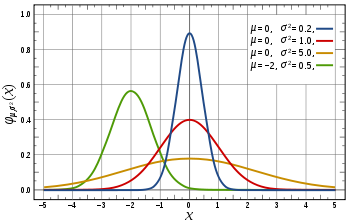
\includegraphics[width=0.9\textwidth]{./imgs/normaldist.png}
	\caption{Função Densidade de Probabilidade de Distribuição Normal.}
	\label{fig:normaldist}
	\fonte{\cite{wikinormaldist}}
\end{figure}

Na Teoria das Probabilidades, o Teorema do Limite Central afirma que, dada certas condições, a média de um número suficientemente grande de variáveis aleatórias independentes, cada uma com média e variância finita, seguirá uma distribuição normal \cite{teoremalimitecentral}.

Em teoria, uma variável aleatória seguindo uma distribuição normal pode assumir valores infinitos, o que é inconveniente computacionalmente. Desta forma, é bastante comum aplicar-se o truncamento desta distribuição, em que um limite inferior e/ou superior é utilizado para adequar os resultado a um intervalo desejado.

Existem algumas formas de se construir computacionalmente um gerador aleatório que segue uma distribuição normal. Dois métodos bastante conhecidos são: transformada de Box-Mueller e algoritmo de Ziggurat.

A transformada de Box-Mueller se baseia num gerador aleatório com distribuição uniforme pode ser expresso em duas formas: a básica e a polar. Na primeira, o gerador uniforme deve gerar valores no intervalo (0, 1], na segunda forma devem ser gerados valores no intervalo [-1, +1] como valores de entrada \cite{boxmueller}.

Supondo que \(U_{1}\) e \(U{2}\) são variáveis aleatórias com distribuição uniforme no intervalo (0, 1] (ou seja, forma básica), as variáveis \(Z_{0}\) e \(Z_{1}\), dadas conforme as equações a seguir, seguirão uma distribuição normal com desvio padrão igual a 1.

Equações:
\[Z_{0} = R\cos{(\Theta)} = \sqrt{-2\ln{U_{1}}}\cos{(2\pi U_{2})}\]
\[Z_{1} = R\sin{(\Theta)} = \sqrt{-2\ln{U_{1}}}\sin{(2\pi U_{2})}\]

A forma polar da transformada pode ser calculada conforme as equações a seguir. Nesta forma, a vantagem reside no fato de que as funções trigonométricas não precisam ser calculadas diretamente \cite{wikiboxmueller}. Considerando que u e v são variáveis uniformemente distribuídas,  e \(s = u^{2} + v^{2}\), as variáveis \(z_{0}\) e \(z{1}\) seguirão uma distribuição normal:

\[z_{0} = \sqrt{-2\ln{U_{1}}}\cos{(2\pi U_{2})} = \sqrt{-2\ln{s}}(\frac{u}{\sqrt{s}})\cos{(2\pi U_{2})}) = u\sqrt{\frac{-2\ln{s}}{s}}\]
\[z_{1} = \sqrt{-2\ln{U_{1}}}\sin{(2\pi U_{2})} = \sqrt{-2\ln{s}}(\frac{v}{\sqrt{s}})\cos{(2\pi U_{2})}) = v\sqrt{\frac{-2\ln{s}}{s}}\]

As condições de validade são: garantir que s seja maior que zero e menor que um. Caso alguma destas condições seja violada, deve-se gerar novos valores de u e v até que as condições sejam satisfeitas.

O Algoritmo Ziggurat se baseia, assim como a transformada Box-Mueller em sua forma polar, no algoritmo de rejeição para gerar valores. Normalmente é utilizado quando a geração de uma grande quantidade de números é necessária \cite{ziggurat}. 

\subsection{Distribuição Triangular}

Esta distribuição, como o nome diz, tem formato triangular. Sua função densidade de probabilidade varia de acordo com três parâmetros: a, b e c, como pode ser observado nas equações a seguir e na Figura \ref{fig:triangulardist}.

\[\left\{\begin{array}{l l}
0 & \mbox{para } x < a \\ 
\frac{2(x-a)}{(b-a)(c-a)} & \mbox{para } a \leqslant x \leqslant c, \\
\frac{2(b-x)}{(b-a)(b-c)} & \mbox{para } c \leqslant x \leqslant b, \\
0 & \mbox{para } b < x
\end{array}\right.\]

\begin{figure}[!htb]
	\centering
	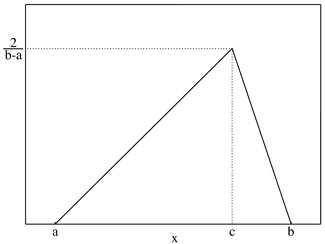
\includegraphics[width=0.9\textwidth]{./imgs/triangulardist.png}
	\caption{Função Densidade de Probabilidade de Distribuição Triangular.}
	\label{fig:triangulardist}
	\fonte{\cite{wikitriangulardist}}
\end{figure}

Computacionalmente é possível criar um gerador aleatório que segue esta distribuição a partir de um gerador aleatório que siga uma distribuição uniforme no intervalo (0, 1) através das equações a seguir:

\[\left\{\begin{array}{l l}
X = a +\sqrt{U(b-a)(c-a)} & \mbox{para } 0 < U < F(c)\\ 
X = b - \sqrt{(1-U)(b-a)(b-c)} & \mbox{para } F(c) \leqslant U < 1
\end{array}\right.\]

\section{Trabalhos Relacionados}

Dada a escala e a complexidade do problema é natural que existam diversos estudos na área, e portanto, existam ferramentas para esse propósito. 
Um breve levantamento pode destacar duas ferramentas desenvolvidas no meio acadêmico que possuem finalidades similares à proposta neste projeto, além de uma no âmbito comercial.

A primeira delas é a MSU \emph{Video Quality Measurement Tool}, desenvolvida pelo grupo do laboratório \emph{Graphics and Media Lab} da \emph(Moscow State University) (MSU) \cite{moscowuniversity}.
A ferramenta tem o propósito de avaliar a qualidade de vídeos se utilizando de métricas objetivas. 
O sistema implementa 20 métricas objetivas, suporta os mais populares formatos de vídeo disponíveis e oferece resultados sumarizados em formato CSV ou um vídeo de vizualização normalizada.
Outra ferramenta é o EvalVid, desenvolvido pelo \emph{Telecommunication Networks Group (TKN)} da \emph{Techinical University of Berlin} \cite{tuberlin}.
Esta se propõe a avaliar a qualidade de vídeos transmitidos por meio de uma rede de comunicação, seja ela simulada ou real, fornecendo parâmetros de qualidade de serviço assim como calculo do PSNR \emph{frame} a \emph{frame}.

O \emph{Picture Quality Analysis System} PQA600 da Tektronix promete avaliações de vídeo digital por meio de métricas objetivas que correspondem fortemente à avaliação visual humana \cite{tektronix}.
O PQA600 é comercializado na forma de uma \emph{workstation} completa, possuindo um poderoso processador, dispositivo de exibição de vídeo e também \emph{interfaces} de captura de vídeo digital e analógico.

\section{Resumo e Conclusão do Capítulo}

Comparando-se as metodologias, ambas são importantes e ambas têm suas limitações. A avaliação objetiva é mais precisa considerando que ela avalie a diferença entre um vídeo original e o efetivamente observado. Porém, nem sempre o vídeo original possui uma qualidade que satisfaria o telespectador, sendo esta, portanto, uma de suas desvantagens.

A avaliação subjetiva embora seja um processo mais difícil de ser realizado por depender de um grande grupo de pessoas e tenha um custo mais elevado \cite{albini}, segundo \cite{wangbovik2004} esta é o tipo de avaliação mais ‘correta’, pois o próprio telespectador realiza a avaliação.
